\chapter{Navier-Stokes Equations - Part 2}
\label{ch:nsderive2}

\section{Significance of the linear relation and Viscosity}

The linear relation between the deviatoric stress tensor and the strain rate tensor (velocity gradient) is physically meaningful for a large number of fluids. Consider the two dimensional case of pure shear stress applied on a layer of liquid. Newton has observed that the shear stress is directly proportional to the velocity gradient.

\index{Newtonian fluid}
\begin{equation}
d_{12} = d_{21} = \mu \frac{\partial u_1}{\partial x_2} 
\end{equation} 

The proportionality constant $\mu$ is {\em defined} as the {\bf viscosity} of the liquid. Fluids that obey this linear relation are called {\em Newtonian fluids}. Examples are water, air and most gases (in most of the situations except under shock wave) and liquid metals. 


Based on their viscosity and the way they flow, materials can be classified as follows:

\begin{figure}[h]
 \centering
 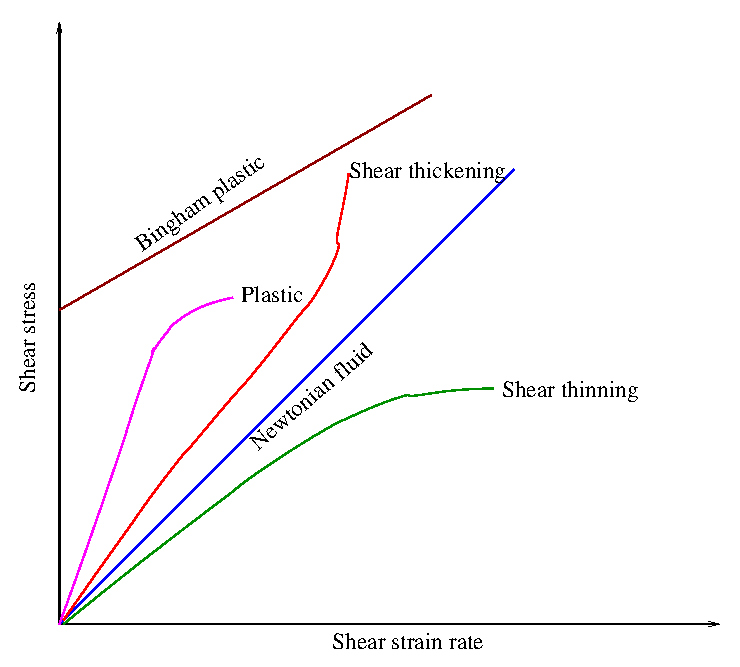
\includegraphics[width=5 in]{images/c10-fluidtypes.eps}
 % ctrans.eps: 46x0 pixel, 300dpi, 0.39x0.00 cm, bb=0 35 595 420
 \caption{Types of fluids}
 \label{fluidtypes}
\end{figure}

% learning objective
\begin{lo2}[Fluid Flow]
  List different types of fluids in contrast with Newtonian fluid
\end{lo2}

\begin{description}

\item[Newtonian fluid]: Strain rate or velocity gradient is linearly dependent on the shear stress as $\sigma_{12}=\mu u_{1,2}$. Eg: air and most of the gases, water, oils of low molecular weight and liquid metals. Often $\sigma_{12}$ is referred to as $\tau_{xy}$.

\item[Bingham Plastic]: Flow starts above a critical shear stress which is then linear with the strain rate. $\sigma_{12}= \sigma_{0} + \mu u_{1,2}$. Eg: drilling muds, peat slurries, margarine, chocolate mixtures, greases, soap, grain-water suspensions, toothpaste, paper pulp, and sewage sludge.

\item[Pseudoplastic]: Shear thinning material - viscosity decreases at higher strain rate. 

\item[Dilatant]: Shear thickening material - viscosity increases at higher strain rate.

\item[Thixotropic]: Viscosity decrease with time.

\item[Rheopectic]: Viscosity increases with time.

\item[Viscoelastic]: The material returns back to its original shape after the stress is removed.

\end{description}


\index{Viscosity}
Viscosity is a strong function of temperature. In liquid metals viscosity follows an {\em Arrhenius} relation. 
In situations where the temperature is roughly constant through out the flow, viscosity can be taken as constant. 
For fluids such as air and water, viscosity is negligible for most of the situations. Such fluids are called {\em inviscid}.  \index{Inviscid fluid}


\section{Reynold's number}

Consider the characteristic length scale of a domain to be $L$. This could be the diameter of a tube through which the fluid flows, the length along a plate over which the fluid flows, the separation between two walls between which the fluid flows and so on. Let $U_0$ be the characteristic velocity. This could be the maximum or average or externally imposed velocity. The characteristic time scale would then be $L/U_0$. Using these, the Navier-Stokes equation can be non-dimensionalized as follows. We take $x_1^* = {x_1 / L}$ as non-dimensionalized distance, $t^* = {t U_0 / L}$ as non-dimensionalized time etc. The non-dimensional velocities are $u_1^* = {u_1/U_0}$ etc.

$$ {\partial \over \partial x_1} = {\partial \over \partial x_1^*} {1 \over L}$$ 
$$ {\partial \over \partial t} = {\partial \over \partial t^*} {U_0 \over L}$$ 

Substitute these into the equation~\ref{nsa1} to obtain:

\begin{equation}
{U_0^2 \over L} \left[  \frac{\partial u_1^*}{\partial t^*} + u_1^* \frac{\partial u_1^*}{\partial x_1^*} + u_2^* \frac{\partial u_1^*}{\partial x_2^*} + u_3^* \frac{\partial u_1^*}{\partial x_3^*} \right] = F_1 -  \frac{1}{\rho L} \frac{\partial p}{\partial x_1^*} + \frac{\nu U_0}{L^2} \left( \frac{\partial^2 u_1^*}{\partial {x_1^*}^2} + \frac{\partial^2 u_1^*}{\partial {x_2^*}^2} + \frac{\partial^2 u_1^*}{\partial {x_3^*}^2} \right)
\end{equation} 

Gather the terms to obtain:

\begin{equation}
\frac{\partial u_1^*}{\partial t^*} + u_1^* \frac{\partial u_1^*}{\partial x_1^*} + u_2^* \frac{\partial u_1^*}{\partial x_2^*} + u_3^* \frac{\partial u_1^*}{\partial x_3^*} = \frac{L}{U_0^2} F_1 -  \frac{1}{\rho U_0^2} \frac{\partial p}{\partial x_1^*} + \frac{\nu}{L U_0} \left( \frac{\partial^2 u_1^*}{\partial {x_1^*}^2} + \frac{\partial^2 u_1^*}{\partial {x_2^*}^2} + \frac{\partial^2 u_1^*}{\partial {x_3^*}^2} \right)
\end{equation} 

Now we can consider that $U_0^2 / L$ as the scaling factor for $F_1$ so that non-dimensional force $F_1^* = {F_1 L / U_0^2}$. Similarly, the scaling factor for pressure can be taken as $\rho U_0^2$ so that non-dimensional pressure $p^* = {p / {\rho U_0^2}}$.


\begin{equation}
\frac{\partial u_1^*}{\partial t^*} + u_1^* \frac{\partial u_1^*}{\partial x_1^*} + u_2^* \frac{\partial u_1^*}{\partial x_2^*} + u_3^* \frac{\partial u_1^*}{\partial x_3^*} = F_1^* -  \frac{\partial p^*}{\partial x_1^*} + \frac{\nu}{L U_0} \left( \frac{\partial^2 u_1^*}{\partial {x_1^*}^2} + \frac{\partial^2 u_1^*}{\partial {x_2^*}^2} + \frac{\partial^2 u_1^*}{\partial {x_3^*}^2} \right)
\end{equation} 

The scaling factor for the diffusive term in the above equation can be taken as follows:

\begin{equation}
\boxed{ 
Re_L \equiv {L U_0 \over \nu} \equiv {L U_0 \rho \over \mu}
}
\end{equation}

Thus the non-dimensionalised Navier-Stokes equation for incompressible Newtonian fluid comes to be:

\begin{equation}
\frac{\partial u_1^*}{\partial t^*} + u_1^* \frac{\partial u_1^*}{\partial x_1^*} + u_2^* \frac{\partial u_1^*}{\partial x_2^*} + u_3^* \frac{\partial u_1^*}{\partial x_3^*} = F_1^* -  \frac{\partial p^*}{\partial x_1^*} + \frac{1}{Re_L} \left( \frac{\partial^2 u_1^*}{\partial {x_1^*}^2} + \frac{\partial^2 u_1^*}{\partial {x_2^*}^2} + \frac{\partial^2 u_1^*}{\partial {x_3^*}^2} \right)
\end{equation} 

The Reynold's number \index{Reynolds number} $Re_L$ is now a measure of the importance of the diffusive term in the Navier-Stokes equation while determining the fluid flow evolution. In the limit of $Re_L \to 0$ the flow field is expected to be governed mainly by the diffusive term. 


The subscript used with Reynold's number will be indicative of the characteristic length scale. A bar on the top, like $\bar{Re}$ indicates the use of average velocity for non-dimensionalization. 

% --------- end of nsderive2.tex ---------------------------------
